\section{Létező megoldások}
\begin{frame}{Létező megoldások}
\framesubtitle{Statistical machine translation}
	
	\begin{figure}[t]
		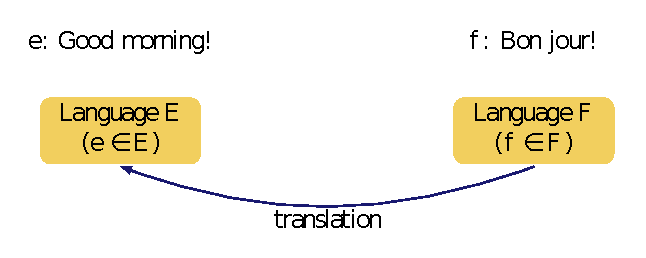
\includegraphics[width=1\linewidth]{images/smt_translation}
 	\end{figure}

	\begin{equation}
		P(e|f) = \frac{P(e)P(f|e)}{P(f)}
	\end{equation}
	\begin{equation}
		T(e) = \hat{e} = argmax_e P(e|f) = argmax_e P(e) P(f|e)
	\end{equation}
	
	
\end{frame}

\begin{frame}{Létező megoldások}
\framesubtitle{Statistical machine translation}

	\begin{align*}
		T(e) = \hat{e} = argmax_e P(e) P(f|e)
	\end{align*}
	
	\begin{itemize}

		\item
			nyelvi modell: $P(e)$
			\begin{itemize}
				\item
					folytonosságot biztosít a célnyelvben
			\end{itemize}

		\item
			fordítási modell: $P(f|e)$
				\begin{itemize}
					\item
			 			lexikális megfeleltetés a nyelvek között
			 		\item
			 			szó alapú (word based) modellek \cite{Brown:1990} \cite{Berger:1994}
			 		\item
			 			kifejezés alapú (phrase based) modellek \cite{Och99improvedalignment} \cite{Marcu:2002}
			 	\end{itemize}
		\item
			argmax: $argmax_e$
			\begin{itemize}
				\item
					keresés
			\end{itemize}
	\end{itemize}
	
	
\end{frame}

\begin{frame}{Létező megoldások}
	\framesubtitle{Előnyök, hátrányok}
	
	Szó alapú vs. kifejezés alapú modellek: 
	\begin{itemize}
		\item
			szó alapú modell: nehéz a tokenizálás \cite{Lopez07asurvey}
		\item
			kifejezés alapú modell pontosabb komplex nyelvek esetén \cite{Lopez07asurvey}
		
	\end{itemize}
	
	Ezen rendszerek hátrányai:
	\begin{itemize}
		\item
			Még mindig nem elég pontosak az SMT-rendszerek a WSD-hez képest \cite{Carpuat_evaluatingthe}
	\end{itemize}
	
\end{frame}


\begin{frame}{Létező megoldások}
	\framesubtitle{Aktuális próbálkozások a javításra}
		
		A lexikális pontosság növelése a legnagyobb kihívás a jelenlegi SMT-rendszerekben!
		
	\begin{itemize}
		\item
			általános Senseval WSD használata \cite{carpuat2005}
		\item
			egyszavas WSD használata jelentés-egyértelműsítésre kifejezés alapú modelleknél \cite{Carpuat06towardintegrating}
		\item
			WSD használata jelentés-egyértelműsítésre többszavas kifejezés alapú modellekre \cite{Carpuat07improvingstatistical}
		
	\end{itemize}
\end{frame}


